\subsection{Směrování} 
Směrování (routování) označuje v informatice určování cest datagramů v prostředí počítačových sítí. Směrování zajišťují nejen routery, ale i koncové stanice (při vysílání) a jejich úkolem je doručit datagram (resp. paket) adresátovi, pokud možno co \textbf{nejefektivnější cestou}. Směrování zajišťuje \textbf{síťová vrstva} modelu ISO/OSI a je využíváno v lokálních sítích LAN i na Internetu, kde jsou dnes směrovány zejména \textbf{IP packety}.

Síťová infrastruktura mezi odesílatelem a adresátem paketu může být velmi složitá, a proto se směrování zpravidla nezabývá celou cestou paketu, ale řeší vždy \textbf{jen jeden krok}, tj. komu datagram předat jako dalšímu. Hledání cesty v síti:

\begin{itemize}
	\item Ve \textbf{spojově orientovaných sítích} (jednobodové, vícebodové) při vytváření spojení:
	\begin{itemize}
		\item Nastavování \textbf{spojovacích polí přepínacích prvků} na cestě.
		\item Budování \textbf{přepínacích tabulek} virtuálního kanálu.
	\end{itemize}
	\item V sítích s \textbf{přepínáním paketů} (obvykle obecně polygonálních a s alternativními cestami) při přenosu každého jednotlivého paketu => \textbf{každý paket může jít jinou cestou}.
\end{itemize}

\subsubsection{Směrování v počítačových sítích a v Internetu}
Abychom mohli paketovou sítí směrovat pakety od zdroje k cíli, potřebujeme správným způsobem naplnit \textbf{směrovací tabulky} všech směrovačů na trase. V malých sítích nebo v sítích, z nichž veškerý provoz ven odchází po jediné implicitní (default) cestě, toto lze vyřešit manuálním vložením potřebných informací, tj. \textbf{statickým směrováním}. V rozlehlejších sítích s měnící se topologií (z nichž největší je bezesporu Internet) jsou však nutné \textbf{dynamické směrovací protokoly}, které zajistí správné naplnění směrovacích tabulek automaticky na základě výměny informací mezi směrovači.

\subsubsection{Neadaptivní -- Statické směrování}
\begin{itemize}
\item \textbf{Směrovací tabulky} v jednotlivých směrovačích \textbf{konfigurovány "ručně"} - pracnější.
\item Odpadá \textbf{režie směrovacích protokolů} (zabraná šířka pásma, čas na zpracování).
\item \textbf{Bezpečnější} (omezení možnosti generování falešných směrovacích informací, odposlouchání topologie sítě).
\item Při \textbf{výpadku} linky nutný \textbf{ruční zásah}.
\item Použitelné, pokud se topologie \textbf{příliš často nemění} (vlivem výpadků a modifikací sítě).
\item V intranetech používáno až překvapivě často.
\end{itemize}

\subsubsection{Adaptivní -- Dynamické směrování}
\begin{itemize}
\item \textbf{Automaticky reaguje} na poměry v síti (topologie, zátěž, ...).
\item Nutnost\textbf{ provozu směrovacích protokolů}.
\item Užitečné \textbf{při častých změnách} (příp. i obecně neznámé) topologie sítě (typicky v Internetu). Algoritmy DVA a LSA
\item V praxi často používána \textbf{kombinace statického a dynamického směrování}, staticky nakonfigurované cesty mají obvykle přednost.
\end{itemize}

\subsubsection{Hierarchické směrování, autonomní systémy}
Současný Internet je natolik \textbf{rozsáhlý} a \textbf{proměnlivý}, že není reálné udržovat ve směrovačích úplnou informaci o jeho topologii. Tato informace by navíc byla velmi nestabilní, protože by se měnila s výpadkem nebo zapojením linky kdekoli na světě. Proto bylo rozhodnuto směrování v Internetu řešit \textbf{hierarchickým způsobem}. Předpokladem jeho použití je rozdělení Internetu do tzv. \textbf{autonomních systémů (AS)}. Autonomním systémem rozumíme souvislou skupinu sítí a směrovačů, které jsou pod společnou správou a řídí se společnou směrovací politikou. Pod společnou směrovací politikou si představme zejména dohodnutý vnitřní směrovací protokol (např. OSPF nebo RIP), ale také speciální požadavky administrátorů na směrování některých druhů provozu (traffic engineering, load balancing). Příkladem autonomního systému tak může být autonomní systém jednoho konkrétního\textbf{ poskytovatele Internetu (ISP)} nebo velké firmy.

Cílem hierarchického směrování je \textbf{vždy nejprve doručit paket} určený pro \textbf{některou ze sítí autonomního systému} na hranice tohoto autonomního systému. O další směrování ke konkrétní síti uvnitř AS se již postará vnitřní směrovací protokol, který topologii (nebo alepoň cesty ke všem sítím) svého vlastního AS zná. Směrovač, který je na hranici autonomního systému a účastní se jak na směrování mezi AS tak ve směrovacím protokolu svého AS, se nazývá \textbf{hraniční směrovač} (angl. border gateway). V případě neznámé cesty, cesta putuje \textbf{default cestou}, která jej pošle nadřazenému AS a ten se o její zpracování dále postará.

\subsubsection{Vnitřní a vnější směrovací protokoly}
Při směrování v rámci jednotlivých autonomních systémů se používají tzv. \textbf{vnitřní směrovací protokoly} - Interior Gateway Protocols, IGP. Naopak pro směrování mezi autonomními systémy se používají \textbf{vnější směrovací protokoly} - Exterior Gateway Protocols, EGP. Typickými vnitřními směrovacími protokoly jsou dnes např. \textbf{OSPF} nebo starší \textbf{RIP}, jako vnější směrovací protokol se používá téměř výhradně protokol \textbf{BGP}.

\subsection{Směrovací algoritmy}
Rozlišujeme dvě základní třídy směrovacích protokolů: protokoly založené na \textbf{vektoru vzdálenosti - DVA}  (distance-vector) a na \textbf{stavech linek - LSA} (link-state). 

\subsection{DVA - Distance Vector}
Sousední směrovače si navzájem vyměňují své směrovací tabulky a doplňují si informace, které se naučí od sousedů, v určitých časových intervalech. \textbf{Topologii} celé sítě však \textbf{neznají}, musí se spokojit s adresami sousedů, přes která mají posílat pakety do jednotlivých cílových sítí a \textbf{vzdálenostmi} k těmto sítím, které společně tvoří tzv. \textbf{distanční vektory}.

\begin{itemize}
\item Na začátku směrovací tabulka obsahuje \textbf{pouze přímo připojené sítě} (staticky nakonfigurováno administrátorem).
\item Směrovače poté \textbf{periodicky zasílají }směrovací tabulky sousedům.
\item Z došlých \textbf{směrovacích tabulek sousedů} (vzdáleností sousedů od jednotlivých sítí) si směrovač postupně \textbf{upravují a budují} svou směrovací tabulku.
\item Pokud cesta \textbf{nebyla delší dobu sousedem inzerována}, ze směrovací tabulky se \textbf{odstraní}.
\end{itemize}

\subsubsection*{Vlastnosti}
\begin{itemize}
\item \textbf{Metrikou} je \textbf{počet "přeskoků"} (hop count) na cestě mezi zdrojem a cílem -- nezohledňuje parametry jednotlivých linek (přenosovou rychlost, zpoždění, okamžitou zátěž, ...).
\item \textbf{Pomalá konvergence při změnách} topologie -- o změně se informuje až při příštím periodickém broadcastu směrovací tabulky.
\item \textbf{Zátěž }od broadcastu celých směrovacích tabulek.
\item \textbf{Příliš "optimistické"} -- směrovač se rychle učí dobré cesty, ale \textbf{špatně zapomíná při výpadcích}.
\begin{itemize}
	\item \textbf{Čekání} na timeout cesty, která přestala být inzerována.
	\item Žádný směrovač nikdy nemá metriku horší, než minimum z metrik sousedů + 1 => pomalé šíření špatných zpráv.
\end{itemize}
\end{itemize}

\subsubsection{Routing information protocol (RIP)}
\begin{itemize}
	\item Velmi starý, stále však \textbf{často implementovaný} v malých sítích.
	\item Hodnota “nekonečna” \textbf{řešící problém počítaní do nekonečna} a v technice Poisson reverse reprezentována číslem 16..
	\item \textbf{Maximální počet} přeskoků je omezen na \textbf{16}.
\end{itemize}

\subsubsection{Interior Gateway Routing Protocol (IGRP)}
\begin{itemize}
\item Cisco proprietary.
\item \textbf{Lepší metrika}, než pouhý počet přeskoků \textbf{bandwidth}, \textbf{delay}, (\textbf{reliability}, \textbf{load}).
\item \textbf{Není omezení }na 16 přeskoků (zvýšeno na 255).
\end{itemize}

\subsection{LSA - Link State}
\begin{itemize}
\item Směrování na základě \textbf{znalosti "stavu" jednotlivých linek sítě} (funkčnost, cena).
\item Směrovače (uzly grafu) \textbf{znají topologii celé sítě }(graf) a \textbf{ceny jednotlivých linek} (ohodnocení hran). Tyto informace udržují v topologické databázi. (Všechny směrovače mají stejnou topologickou databázi).
\item \textbf{Každý směrovač počítá strom nejkratších cest} ke všem ostatním směrovačům (a k nim připojeným sítím) pomocí \textbf{Dijkstrova algoritmu}. (Na rozdíl od DVA všechny směrovače počítají na základě \textbf{stejných} a\textbf{ úplných dat})
\item Každý směrovač\textbf{ neustále sleduje stav} a \textbf{funkčnost} k němu připojených linek.
\item Testováním linek k sousedním směrovačům – \textbf{Hello protokol}.
\item Při \textbf{změně okamžitě šíří informaci} o aktuálním stavu svého okolí všem ostatním směrovačům. Ty si ji vloží do topologické databáze.
\item \textbf{Šíří se pouze změny} (ale do celé sítě) - žádné periodické rozesílání směrovacích tabulek.
\item \textbf{Okamžitá reakce na změnu stavu linek} (výpadek, náběh) => rychlá konvergence
\item Zástupci: \textbf{OSPF (Open Shortest Path First)}
\end{itemize}

\subsection{Adresování} 
Adresování sítě přiděluje oblastní správce (pro Evropu \textbf{RIPE}). IP adresa je \textbf{logická adresa} zařízení v počítačové síti (na 3. vrstvě podle OSI modelu), která používá IP protokol. V IPv4 je tato adresa velká 32bitů (4 byte) a zapisuje se pomocí \textbf{dot-decimal notation}. To znamená pomocí čtyř dekadických hodnot (každá velká jeden byte), označovaných jako oktet, oddělených tečkou. Příkladem IP adresy je 193.222.5.15. 

IP adresa se skládá z několika částí. V základu jde o dvě části, \textbf{prefix} identifikující síť a \textbf{adresa uzlu} v rámci podsítě.

Pro to, abychom určily, která část IP adresy je pro \textbf{podsíť} a která pro \textbf{uzel}, se používá \textbf{maska podsítě} (subnet mask). Ta v binárním tvaru obsahuje jedničky následované nulami a pomocí jedniček\uv{vymaskovává} část síťového prefixu v IP adrese. Jinak řečeno, tam kde jsou v masce jedničky je v IP adrese část podsítě a kde jsou nuly je část uzlu. Síťová část IP adresy určuje podsíť a používá se ke směrování. Část uzlu identifikuje stanici uvnitř daného subnetu.

Maska se v IPv4 zapisuje stejně jako IP adresa pomocí dot-decimal form s tím, že jsou validní pouze adresy, které v binárním zápisu mají zleva jedničky následované nulami (za první nulou smí být pouze nuly). Příkladem síťové masky je 255.255.255.0. Maska 255.255.255.254 není platná, protože uvnitř takového subnetu by se nacházelo 0 uzlů. Maska 255.255.255.255 není maskou podsítě, ale určuje jeden uzel.

Občas se používá speciální zápis, který se označuje jako \textbf{inverse mask} nebo \textbf{wildcard mask}. Jedná se o obrácenou masku, jednoduše řečeno tam, kde jsou v tradiční masce jedničky jsou nuly a naopak. Pro výpočet v dekadické formě můžeme použít pro každý oktet hodnota = 255 – hodnota oktetu. Například pro masku 255.255.255.240 je inversní maska 0.0.0.15.

\begin{figure}[H]
	\centering
	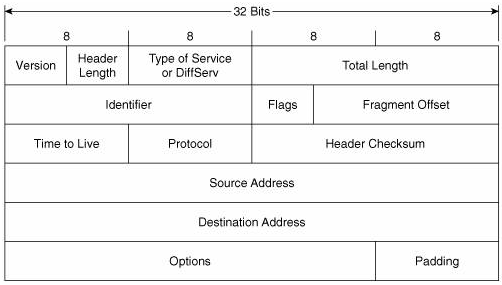
\includegraphics[width=0.7\textwidth]{assets/ipv4-header}
	\caption{Hlavička IPv4}
\end{figure}

\subsubsection{Veřejné a privátní adresy}
Prvotní princip IP sítí byl takový, že IP adresa musela být unikátní v rámci celé sítě a jednotlivé uzly (stanice, servery a další zařízení s přiřazenou IP adresou) spolu mohly komunikovat. S rozvojem internetu se ukázalo, že \textbf{počet adres}, které je možno v IPv4 vytvořit, rozhodně \textbf{není dostatečný}. Začaly se tedy používat různé metody, jak se  s nedostatkem adres vypořádat. Nejrazantnější je nová verze IP protokolu IPv6, která obsahuje mnohem více adres, ale její nasazování není jednoduché. Dále se objevila technika CIDR (Classless Inter-Domain Routing, tj. „beztřídní směrování“ ) a také se IP adresy rozdělili na dva typy, na veřejné a neveřejné IP adresy.

Veřejné IP adresy (public address) tvoří hlavní část adresního rozsahu internetu a tyto adresy jsou routovatelné v rámci celého internetu. Jednoduše řečeno počítač s veřejnou adresou může být dostupný z celého internetu. Tyto adresy musí být unikátní v celé síti (internetu).

Oproti tomu privátní IP adresy (private adress) by se měly používat pouze v rámci LAN sítí a v internetu by přes ISP neměli komunikovat. Firma pak používá jednu (nebo více) veřejnou adresu a pomocí techniky NAT (Network Address Translation) se při komunikaci mimo LAN překládají privátní adresy na tuto veřejnou. Stejné privátní adresy se tak mohou nacházet na mnoha místech v internetu, ale nemohou spolu přímo komunikovat. Následující tabulka ukazuje jednotlivé privátní rozsahy.
\begin{figure}[H]
\centering
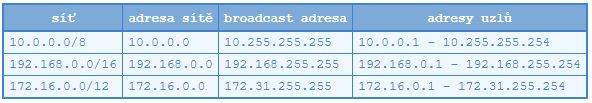
\includegraphics[width=1\textwidth]{assets/6_ip4}
\end{figure}

IP adresy se dělí na:
\begin{itemize}
\item \textbf{unicast} -- adresa jednoho konkrétního počítače,
\item \textbf{multicast} -- adresa pro více počítačů najednou,
\item \textbf{broadcast} -- adresa na všechny počítače. Šíří se jen v rámci segmentu počítače, dál není propuštěna (255.255.255.255).
\item \textbf{loopback} -- zpětnovazební adresa, pošle paket zpátky na vlastní počítač (127.0.0.1).
\end{itemize}

\subsection{IPv6}
IPv6 \textbf{nahrazuje} dosluhující protokol IPv4. Přináší zejména \textbf{masivní rozšíření adresního prostoru} a zdokonalení schopnosti přenášet \textbf{vysokorychlostně data}. Starší protokol IPv4 poskytuje omezený adresní prostor – teoreticky $2^{32}$ adres. IPv6. Obsahuje celkem $2^{128}$ adres. Většina přenosových a aplikačních vrstev protokolů vyžaduje malé nebo žádné změny pro funkčnost s IPv6. Výjimkami jsou protokoly aplikací zahrnující adresy síťové vrstvy např.: FTP. \textbf{Multicast} je součástí základní specifikace IPv6 na rozdíl od IPv4, kde byl zaveden později. IPv6 nepoužívá \textbf{broadcast} na místní linku. Každá adresa má \textbf{128b}. \textbf{Odstraněna potřeba NAT}. Protokol pro IP vrstvu šifrování a autentizaci \textbf{IPsec} je integrální součástí souboru protokolů IPv6, na rozdíl od IPv4, kde je přítomen volitelně (obvykle ale implementován).

IPv6 adresy se obvykle zapisují jako osm skupin čtyř hexadecimálních číslic: \textbf{2001:0db8::1428:57ab}. Vzhledem k zdlouhavému zápisu se může \textbf{nejdelší sekvence nul} nahradit \textbf{::}, \textbf{4 nuly můžeme nahradit jednou}.

\subsubsection{IPv6 Packet}
Paket IPv6 se skládá ze dvou hlavních částí: hlavičky a těla.
\begin{itemize}
	\item \textbf{Verzi} - 4 bity, verze 6
	\item \textbf{Dopravní třídu} - 8 bitů na prioritu paketu. Úroveň priority se dělí na rozsahy: kde zdroj podporuje kontrolu přetížení a bez podpory kontroly přetížení.
	\item \textbf{Pojmenování toku} - 20 bitů pro správu QoS. Původně určeno pro speciální obsluhu aplikací reálného času, nyní se nepoužívá.
	\item \textbf{Délka těla} - 16 bitů pro délku těla paketu. Při vynulování se nastaví „jumbo“ tělo (skok za skokem).
	\item \textbf{Následující hlavička} - 8 bitů, určuje další vnořený protokol. Hodnoty se shodují s hodnotami definovanými pro IPv4.
	\item \textbf{Zdrojová a cílová adresa} - 128 bitů na každou adresu.
	\item\textbf{Hop limit }- 8 bitů, číselně definuje počet povolených přechodů síťovými prvky. Každý přechod znamená snížení čísla o 1.
\end{itemize}

\begin{figure}[H]
	\centering
	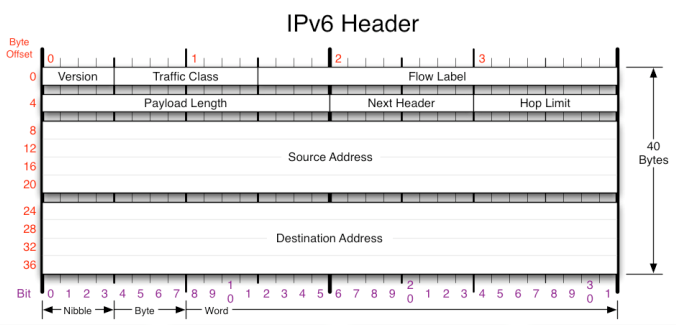
\includegraphics[width=\textwidth]{assets/4_ipv6}
\end{figure}


\subsection{Překlad síťových adres NAT}
\textbf{NAT (Network address translation)} se většinou používá pro přístup více počítačů z \textbf{lokální sítě} na \textbf{Internet} pod \textbf{jedinou veřejnou adresou}. Překládá zdrojovou a cílovou IP adresu, je realizován na \textbf{routerech}, \textbf{firewallech} většinou zařízeních 3 vrstvy. Umožňuje připojit více počítačů na jednu veřejnou IP adresu - řeší se tak nedostatek přidělených veřejných IP adres. Využívá se \textbf{překladové tabulky}. 
\\\\
\textbf{Výhody:} 
\begin{itemize}
	\item Zvyšuje bezpečnost počítačů připojených za NATem (potenciální útočník nezná opravdovou IP adresu). 
	\item Umožňuje připojit více počítačů na jednu veřejnou IP adresu, čímž se obchází nedostatek IPv4 adres
\end{itemize}
\textbf{Nevýhody:}
\begin{itemize}
	\item Zařízení za NATem nemají skutečné připojení k Internetu (není možné se snadno připojit na zařízení za NATem.)
	\item NAT znemožňuje správnou funkcionalitu některých software
\end{itemize}

\subsubsection{Typy NATu}
Typicky se využívá kombinace obou níže zmíněných řešení.
\begin{itemize}
	\item \textbf{Statický NAT} - Překladová tabulka je konfigurována manuálně administrátorem.
	\item \textbf{Dynamický NAT} - Obsah překladové tabulky je vytvářen dynamicky v závislosti na síťovém provozu. Veřejné adresy jsou alokovány jednotlivým spojením jejich vypůjčením z \textbf{NAT Poolu}.
	\item \textbf{Network adress and port translation NAPT} - Několik uzlů využívá pouze jednu veřejnou IP adresu. Jednotlivé uzly jsou identifikovány pomocí různých čísel portů.
\end{itemize}

\begin{figure}[H]
\centering
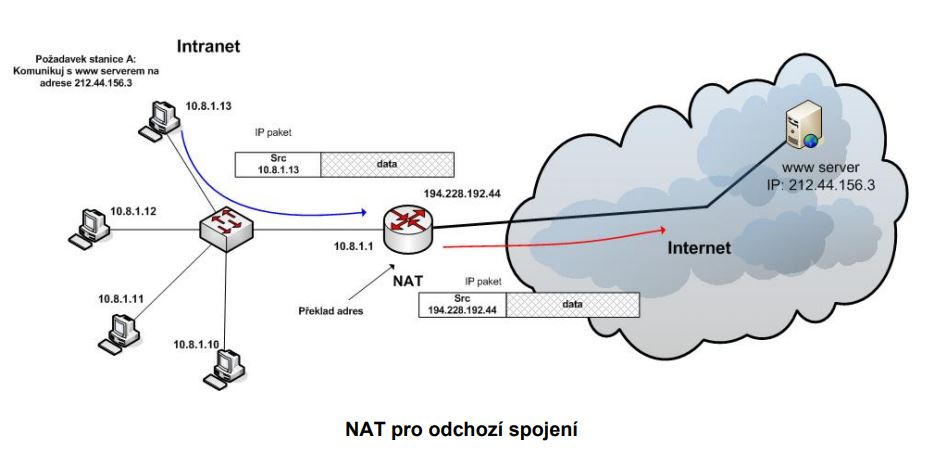
\includegraphics[width=1\textwidth]{assets/6_nat_out}
\end{figure}

\begin{figure}[H]
\centering
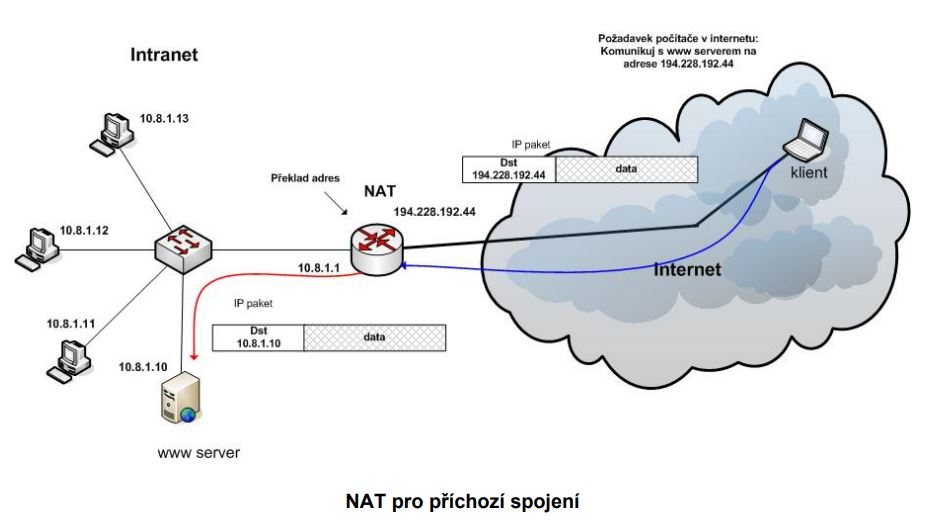
\includegraphics[width=1\textwidth]{assets/6_nat_in}
\end{figure}

\subsubsection{PAT (Port Address Translation)}
V případě PAT dochází k překladu jak adres tak i příslušných portů v IP komunikaci. Výhodou zde je, že za jednu venkovní IP adresu můžeme maskovat celou řadu služeb, které jsou hostovány na různých serverech. Typickým příkladem jsou FTP a www servery umístěné v DMZ. 
\begin{figure}[H]
\centering
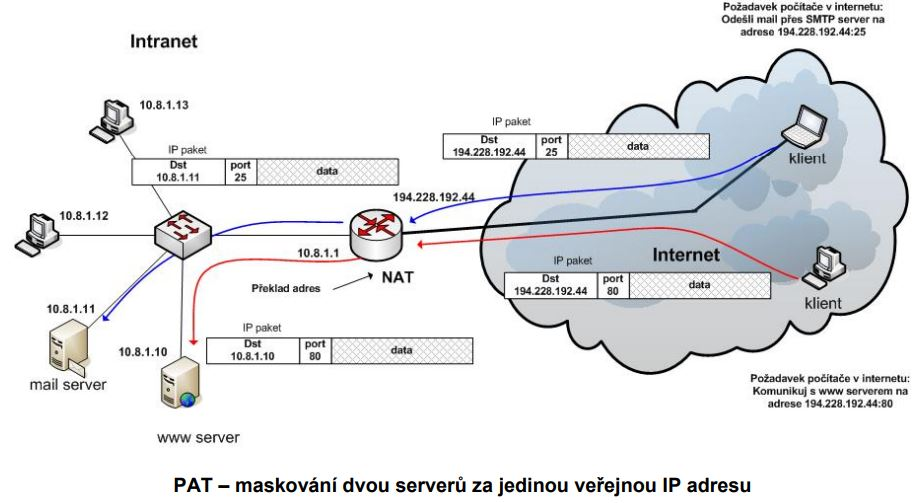
\includegraphics[width=1\textwidth]{assets/6_pat_mask}
\end{figure}